\chapter{WAMIT2 Module Architecture}
\label{chap:architecture}
\todo[inline]{This section is copied from the old writeup.  {\textbf{It has not been updated.}}}
\todo[inline]{Add in the registry infromation as needed}

Figure 1 shows the development architecture of the WAMIT2 module for HydroDyn. Once it has been developed, this module will eventually be incorporated into HydroDyn. During development, it will interface with its driver routine which will mimic the interface of the HydroDyn module. Because there is ongoing development in the existing HydroDyn modules, a copy of the modularized Waves sub-module (Waves2) will be used and converted to handle bi-directional waves. This will be merged back into the Waves module later.

\begin{figure}
   \centering
      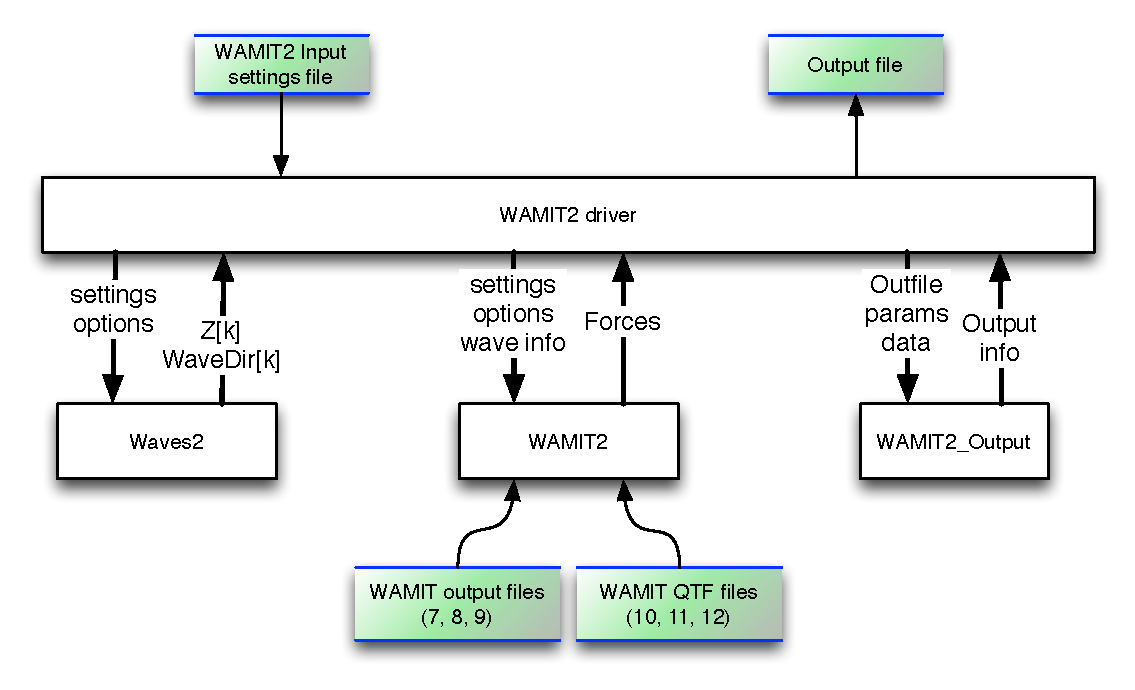
\includegraphics[width=.9\textwidth]{chaps/figures/WAMIT2_Dev.pdf}
      \caption{Information flow to and from the WAMIT2 module. The green boxes indicate information or files passed into or out of the module.\label{fig:W2Interface}}
\end{figure}


\endinput


\begin{figure}
   \centering
      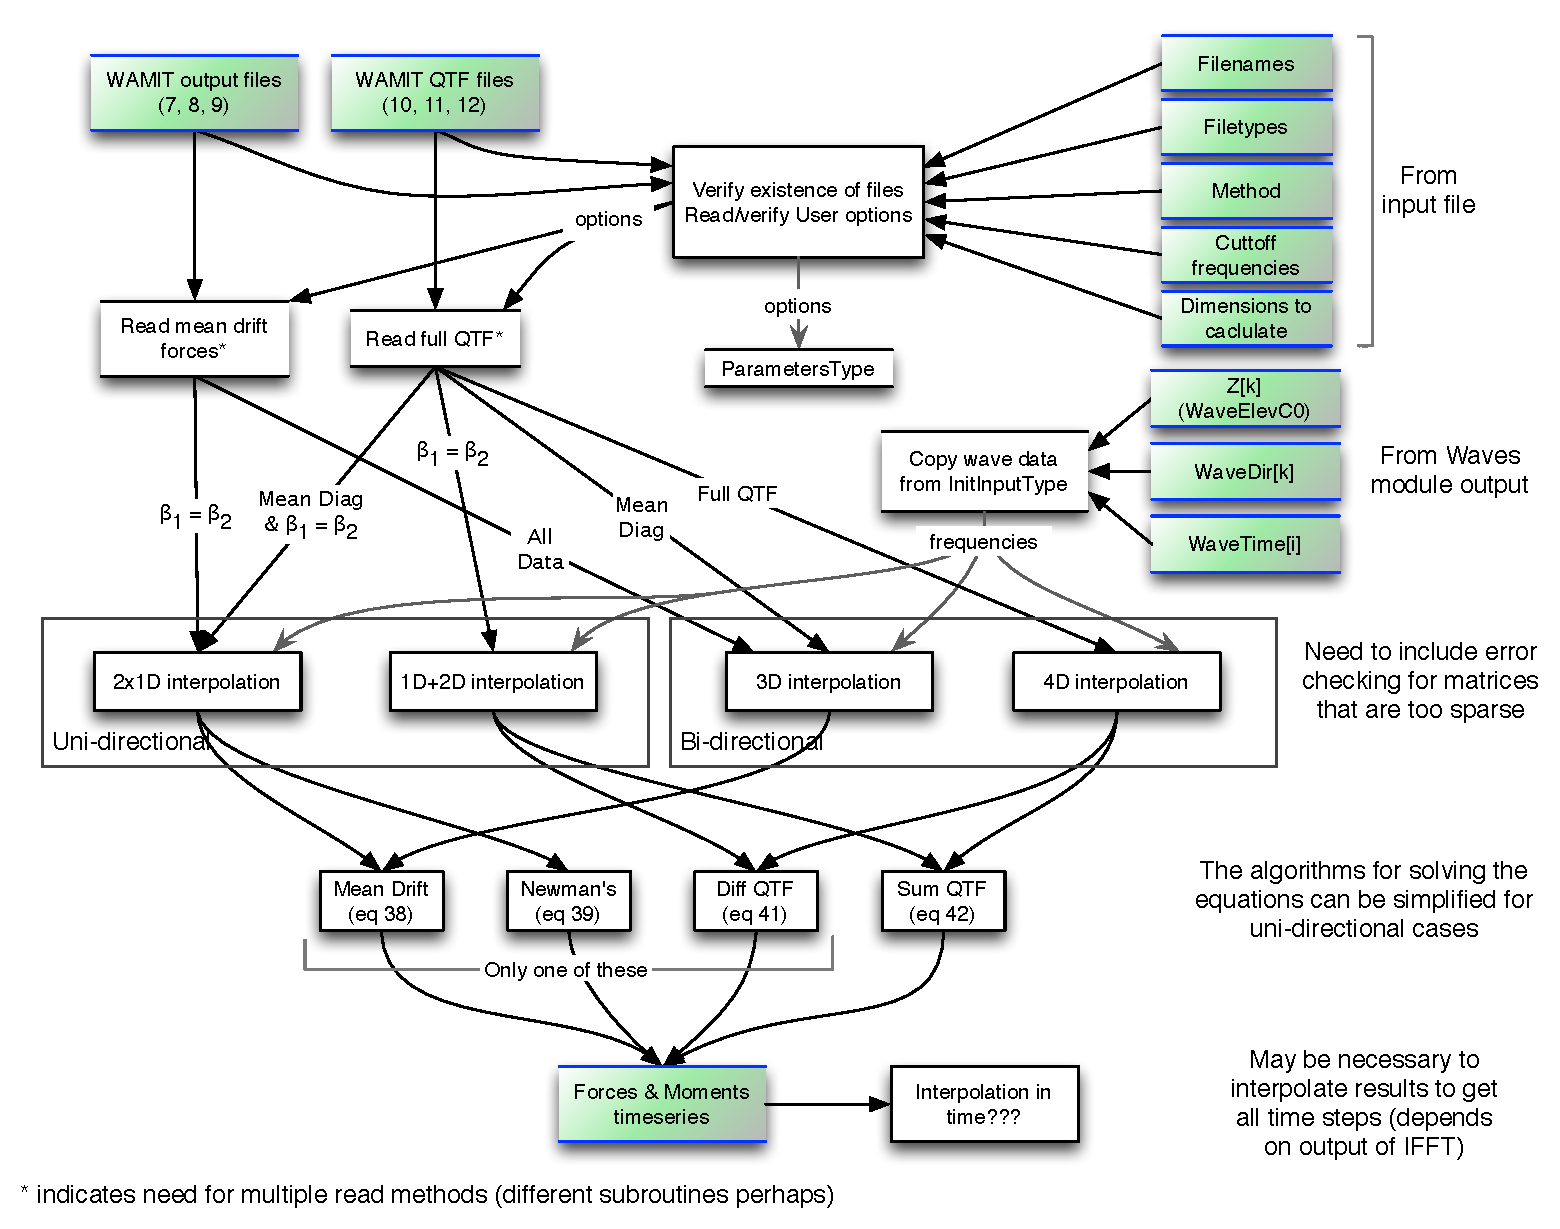
\includegraphics[width=.9\textwidth]{chaps/figures/HydroDyn_2nd_order--WAMIT2_Init.pdf}
      \caption{Information flow within the Init routine in the WAMIT2 sub-module. {\bfseries OUTDATED:} Diagram for parse then interpolate method -- interpolation is done at each step in the equation solver using a 3D and 4D interpolation.\label{fig:InitInformationFlow}}
\end{figure}

\section{Input information}
The wave information in the frequency domain will need to be passed into the WAMIT2 module. This is available at the platform reference point as \emph{WaveElevCO} in the \emph{InitOutputType} from the Waves module (calculated on line 1322 of \emph{Waves.f90}, revision 98 in \emph{branches/HydroDyn\_Modularization/Source}). In the code, the frequency is given as $\omega = k \Delta \omega$, the index times the frequency step. Since $k$ is positive, there are no negative frequencies. Tiago assumed in equation 23 of his write-up that there are negative frequencies, so I assume he included them simply for completeness (I don't think it makes sense to worry about negative frequencies since that can be accounted for by direction).

At present, the Waves module only uses a single direction for the waves. So, an array of wave directions does not exist (scalar value at present). That will need to be added to the Waves module at some point.

\section{File reading}
The WAMIT files to be read in can have an extension of .7, .8, .9, .10d, .10s, .11d, .11s, .12d, or .12s. The .7 extension is only available for files generated with WAMIT 7, not WAMIT 6.1s or 6.4, so that may need to be checked.
The entirety of the files is read in and stored in memory.  This involves several passes through the file to figure out how frequency and wave direction components are present in the file, allocate the storage, then read everything in at once.

\section{Calculations}
The calculations are outlined elsewhere in this document.

\section{Init returned information}
%FIXME: Jason thinks this should be $N' = 2(N+1)$ instead of $N$.  I need to double check, but I think my notation has $N'$ and $N$ switched.  I may wish to change this.
The returned information will be an array of forces and moments at specific timesteps (ideally the same as those returned by the WAMIT routine). I suspect that it will be least confusing to return a $6\times N$ array (3 forces, 3 moments, $N$ timesteps) regardless of which forces are calculated. The unrequested ones will just be set to zero. I will have to look at the WAMIT module that Greg worked on to see how he output these forces -- I think they are on a single point mesh.

\section{CalcOutput routine}
This routine will interpolate the force data created by the Init routine in order to get the forces at intermediate timesteps. It may not be necessary to interpolate at all timesteps since the Init routine calculates the forces for all known timesteps at the start of the FAST simulation. However, it might be necessary to interpolate for other timesteps depending on the coupling used in FAST.

\section{HydroDyn modifications/considerations}

\begin{itemize}
   \item{2nd order won't work for certain WaveMod cases because the $Z[k]$ won't be known (i.e. \emph{WaveMod}~$= 5$ for \emph{GH\_BladedWaves\_Init}). Cases to check are \emph{WaveMod} $= \{0,4,5\}$\todo{update from WAMIT.f90}. This should be checked for at the HydroDyn level.  This may need to be checked in {\tt WAMIT2.f90} (it is checked in {\tt WAMIT.f90}).}
\end{itemize}


\endinput
\section{Program Outline}
\subsection{WAMIT2\_Init}
\label{sec:WAMIT2Init}
\todo[inline]{Add in a check on the WaveMod.  See WAMIT.f90 line ~894 ({\tt InitInp\%WaveMod} case)}
\begin{itemize}
   \item{Check inputs}\todo{Change all these to case structures}
   \begin{itemize}
      \item{Values of \emph{MnDrift}, \emph{NewmanApp}, \emph{DiffQTF}, and \emph{SumQTF}}
      \item{Size of \emph{WaveTime}, \emph{WaveElevC0}, and \emph{WaveDir} arrays}
      \item{Cutoff frequencies make sense}
      \item{Existence of WAMIT files}
   \end{itemize}
   \item{Copy input info into WAMIT2\_Parameters}
   \item{Read and parse input files}
   \begin{itemize}
      \item{Mean Drift Force files (\{\emph{MnDrift} || \emph{NewmanApp}\} = \{.7, .8, .9\})}
      \begin{itemize}
         \item{\emph{WaveMultiDir} = .FALSE. $\rightarrow$ $\beta1=\beta2$}
         \item{\emph{WaveMultiDir} = .TRUE. $\rightarrow$ All}
      \end{itemize}
      \item{Difference QTF files (\emph{DiffQTF} = \{.10d, .11d, .12d\})}
      \begin{itemize}
         \item{\emph{WaveMultiDir} = .FALSE.}
         \begin{itemize}
            \item{\emph{MnDrift} || \emph{NewmanApp} $\rightarrow$ Mean diaganoal and $\beta_1 = \beta_2$}
            \item{\emph{DiffQTF} $\rightarrow$ $\beta_1 = \beta_2$}
         \end{itemize}
         \item{\emph{WaveMultiDir} = .TRUE.}
         \begin{itemize}
            \item{\emph{MnDrift} $\rightarrow$   Mean diagonal}
            \item{\emph{DiffQTF} $\rightarrow$   Full QTF}
         \end{itemize}
      \end{itemize}
      \item{Sum QTF files (\emph{SumQTF} = \{.10s, .11s, .12s\})}
      \begin{itemize}
         \item{\emph{WaveMultiDir} = .FALSE. $\rightarrow$ $\beta_1 = \beta_2$}
         \item{\emph{WaveMultiDir} = .TRUE. $\rightarrow$ Full QTF}
      \end{itemize}
   \end{itemize}
   \item{Interpolation}
   \begin{itemize}
      \item{Diff frequency}
      \begin{itemize}
         \item{\emph{WaveMultiDir} = .FALSE.}
         \begin{itemize}
            \item{\emph{MnDrift} || \emph{NewmanApp} $\rightarrow$ 2x1D (\Cref{sec:interp:1d})}
            \item{\emph{DiffQTF} $\rightarrow$   1D+2D (\Cref{sec:interp:1d,sec:interp:2d})}
         \end{itemize}
         \item{\emph{WaveMultiDir} = .TRUE.}
         \begin{itemize}
            \item{\emph{MnDrift} $\rightarrow$   3D (\Cref{sec:interp:3d})}
            \item{\emph{DiffQTF} $\rightarrow$   4D (\Cref{sec:interp:4d})}
         \end{itemize}
      \end{itemize}
      \item{Sum frequency}
      \begin{itemize}
         \item{\emph{WaveMultiDir} = .FALSE. $\rightarrow$  1D+2D (\Cref{sec:interp:1d,sec:interp:2d})}
         \item{\emph{WaveMultiDir} = .TRUE. $\rightarrow$   4D (\Cref{sec:interp:4d})}
      \end{itemize}
   \end{itemize}
   \item{Calculation of forces}
   \begin{itemize}
      \item{\emph{MnDrift} $\ne 0 \rightarrow$     \Cref{eq:MeanDrift}}
      \item{\emph{NewmanApp} $\ne 0 \rightarrow$   \Cref{eq:Newman}}
      \item{\emph{DiffQTF} $\ne 0 \rightarrow$     \Cref{eq:DiffQTF}}
      \item{\emph{SumQTF} $\ne 0 \rightarrow$      \Cref{eq:DiffQTF}}
   \end{itemize}
   \item{Cleanup and exit}
   \begin{itemize}
      \item{Copy data to output mesh}
      \item{Set uncalculated forces to zero}
      \item{Deallocatetemporaryarrays}
   \end{itemize}
\end{itemize}

\subsection{WAMIT2\_CalcOutput routine}
\begin{itemize}
   \item{Interpolate Forces to time DT (may not always be necessary)}
\end{itemize}

\subsection{WAMIT2\_End}
\begin{itemize}
   \item{Destroy data}
\end{itemize}


